\documentclass[a4paper,12px]{article}

\usepackage{graphicx}
\usepackage[english]{babel}
\usepackage{fancyhdr}
\usepackage{lastpage}
\usepackage{xifthen}
\usepackage[linesnumberedhidden, titlenotnumbered]{algorithm2e}
\usepackage{lipsum}
\usepackage{hyperref}
\usepackage{array}
\usepackage{tabularx}

\usepackage{minted}
\usepackage{caption}
\usepackage{amssymb}

\pagestyle{fancy}
\lhead{
\includegraphics[width=7cm]{logoUvA}}
\rhead{\footnotesize \textsc {Report\\ \opdracht}}
\lfoot
{
    \footnotesize \studentA
    \ifthenelse{\isundefined{\studentB}}{}{\\ \studentB}
    \ifthenelse{\isundefined{\studentC}}{}{\\ \studentC}
    \ifthenelse{\isundefined{\studentD}}{}{\\ \studentD}
    \ifthenelse{\isundefined{\studentE}}{}{\\ \studentE}
}
\cfoot{}
\rfoot{\small \textsc {Page \thepage\ of \pageref{LastPage}}}
\renewcommand{\footrulewidth}{0.5pt}

\fancypagestyle{firststyle}
{
    \fancyhf{}
    \renewcommand{\headrulewidth}{0pt}
    \chead{
\includegraphics[width=7cm]{logoUvA}}
    \rfoot{\small \textsc {Page \thepage\ of \pageref{LastPage}}}
}

\setlength{\topmargin}{-0.3in}
\setlength{\textheight}{630pt}
\setlength{\headsep}{40pt}

% =================================== DOC INFO ===================================

\newcommand{\titel}{MPI}
\newcommand{\opdracht}{Assignment 3.2: Collective Communication}
\newcommand{\docent}{Dr. C. Grelck}
\newcommand{\cursus}{Concurrency and Parallel Programming}
\newcommand{\vakcode}{5062COPP6Y}
\newcommand{\datum}{\today}
\newcommand{\studentA}{Robin Klusman}
\newcommand{\uvanetidA}{10675671}
\newcommand{\studentB}{Maico Timmerman}
\newcommand{\uvanetidB}{10542590}
%\newcommand{\studentC}{Boudewijn Braams}
\newcommand{\uvanetidC}{10401040}
%\newcommand{\studentD}{Govert Verkes}
\newcommand{\uvanetidD}{10211748}
%\newcommand{\studentE}{Naam student 5}
\newcommand{\uvanetidE}{UvAnetID student 5}

% ===================================  ===================================

\begin{document}
\thispagestyle{firststyle}
\begin{center}
    \textsc{\Large \opdracht}\\[0.2cm]
    \rule{\linewidth}{0.5pt} \\[0.4cm]
    {\huge \bfseries \titel}
    \rule{\linewidth}{0.5pt} \\[0.2cm]
    {\large \datum  \\[0.4cm]}

    \begin{minipage}{0.4\textwidth}
        \begin{flushleft}
            \emph{Student:}\\
            {\studentA \\ {\small \uvanetidA \\[0.2cm]}}
            \ifthenelse{\isundefined{\studentB}}{}{\studentB \\ {\small \uvanetidB \\[0.2cm]}}
            \ifthenelse{\isundefined{\studentC}}{}{\studentC \\ {\small \uvanetidC \\[0.2cm]}}
            \ifthenelse{\isundefined{\studentD}}{}{\studentD \\ {\small \uvanetidD \\[0.2cm]}}
            \ifthenelse{\isundefined{\studentE}}{}{\studentE \\ {\small \uvanetidE \\ [0.2cm]}}
        \end{flushleft}
    \end{minipage}
    ~
    \begin{minipage}{0.4\textwidth}
        \begin{flushright}
            \emph{Supervisor:} \\
            \docent \\[0.2cm]
            \emph{Course:} \\
            \cursus \\[0.2cm]
            \emph{Course code:} \\
            \vakcode \\[0.2cm]
        \end{flushright}
    \end{minipage}\\[1 cm]
\end{center}


% =================================== FRONT PAGE ===================================

\vspace{2cm}
\begin{center}
    
\includegraphics[width=(\textwidth/5*3)]{parallel_tasks}
\end{center}
\clearpage

\tableofcontents
\vspace{5mm}

% =================================== MAIN TEXT ===================================

\section{Introduction}

Hadoop is an implementation of MapReduce, that simplifies the usage of MapReduce
greatly. Hadoop requires the user to write his own Map and Reduction function
and deals with the rest of the configuration itself. Hadoop has a built-in
distributed file system,  Hadoop Distributed File System (HDFS).  The HDFS is
accessible from all nodes running Hadoop, making read-write operations very
convenient.

In this program Hadoop is used to process large quantities of data. The data
that will be processed in this case are a collection of tweets from 2009. These
tweets will first be scanned for any hashtags to determine which hashtags were
the most popular ones in this set of tweets. Then for each of the tweets
containing a hashtag the language will be determined. If the language happens to
be English, the sentiment value is calculated and returned to the reduce
function. Finally the mean and standard deviation of the sentiment values will
also be calculated.


\section{Method}

The first thing the program has to do is map the data to the available nodes.
In this case each node gets one line of text from the file that is being read.
The first thing to do when this line of text is received is to check if this is
the line containing the actual tweet, and not the date or URL belonging to a
tweet. If the line is found to be a tweet, the second step is to determine if
this tweet contains any hashtags, and what they are. If there are no hashtags at
all in the tweet, it will be discarded. If there is however a hashtag in the
tweet, we will then determine the language of the tweet. If the language is
found to be English, the sentiment value can finally be calculated. This value
is then returned to the reduce function together with the hashtag(s) that were
in that tweet in a so called key-value pair, where the key is the hashtag and
the value the sentiment (in case there were multiple hashtags in a single tweet,
each one of them is sent in a separate key-value pair).
The reduce function will then determine the mean and standard deviation of the
sentiment value for a specific hashtag and output these.
The image below illustrates the various steps taken in finding the sentiment
value for a specific hashtag/tweet.

\begin{center}
    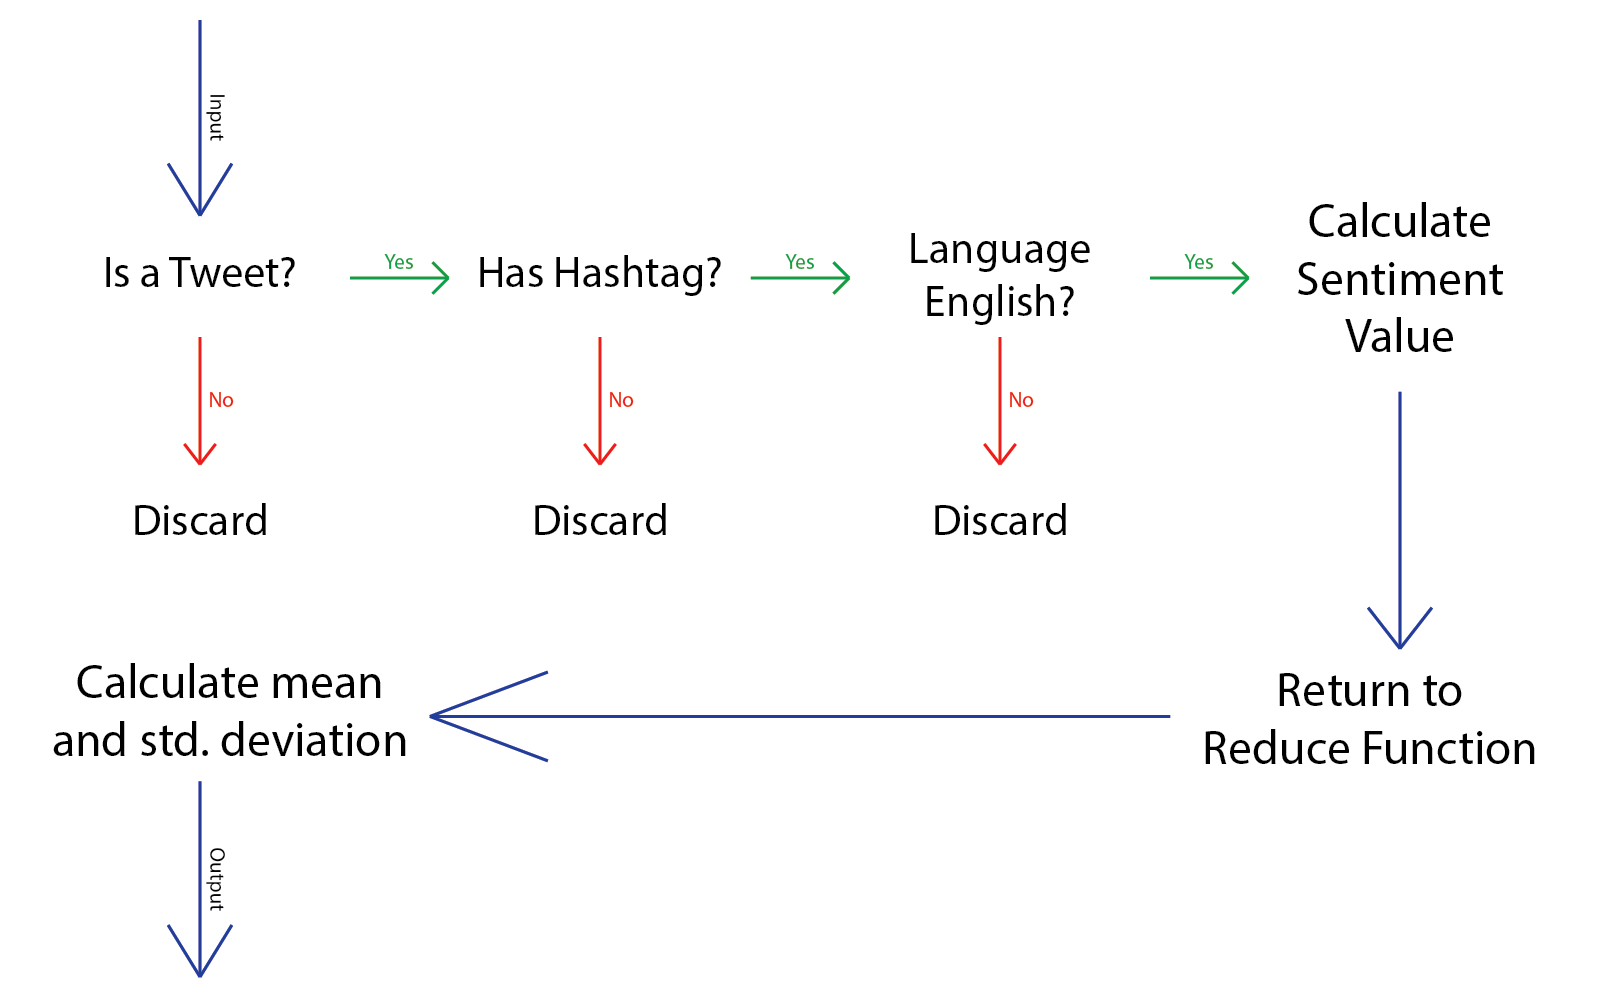
\includegraphics[width=\textwidth]{steps}
\end{center}
\captionof{figure}{Steps taken and checks done in finding the sentiment value
belonging to a certain tweet/hashtag.}

\section{Results}

In this section the results we found are presented. This includes the data we
found when looking for the ten most popular hashtags and their average sentiment
value and standard deviation, in addition to the speed up factor of the program
when using multiple nodes compared to one node. \\

\noindent\begin{tabularx}{\textwidth}{p{.22\textwidth} p{.15\textwidth} p{.25\textwidth} p{.25\textwidth}}
    Hashtag & Occurences & Average Sentiment & Standard Deviation \\
    \hline
    \#iranelection  & 29 & 1.48 & 0.77 \\
    \#tcot          & 10 & 1.80 & 0.87 \\
    \#followadd     & 9  & 2.00 & 0.00 \\
    \#spymaster     & 8  & 1.50 & 0.87 \\
    \#140mafia      & 8  & 2.00 & 1.00 \\
    \#neda          & 7  & 1.57 & 0.73 \\
    \#fb            & 7  & 2.00 & 0.93 \\
    \#jobs          & 6  & 2.50 & 0.50 \\
    \#iran          & 6  & 1.33 & 0.75 \\
    \#forasarney    & 6  & 2.00 & 0.00 \\
\end{tabularx}
\captionof{table}{Top ten hashtags (from English tweets only) with their
    occurences, \\ \hspace{2cm} average sentiment value and standard deviation of the sentiment
value.}

\begin{center}
    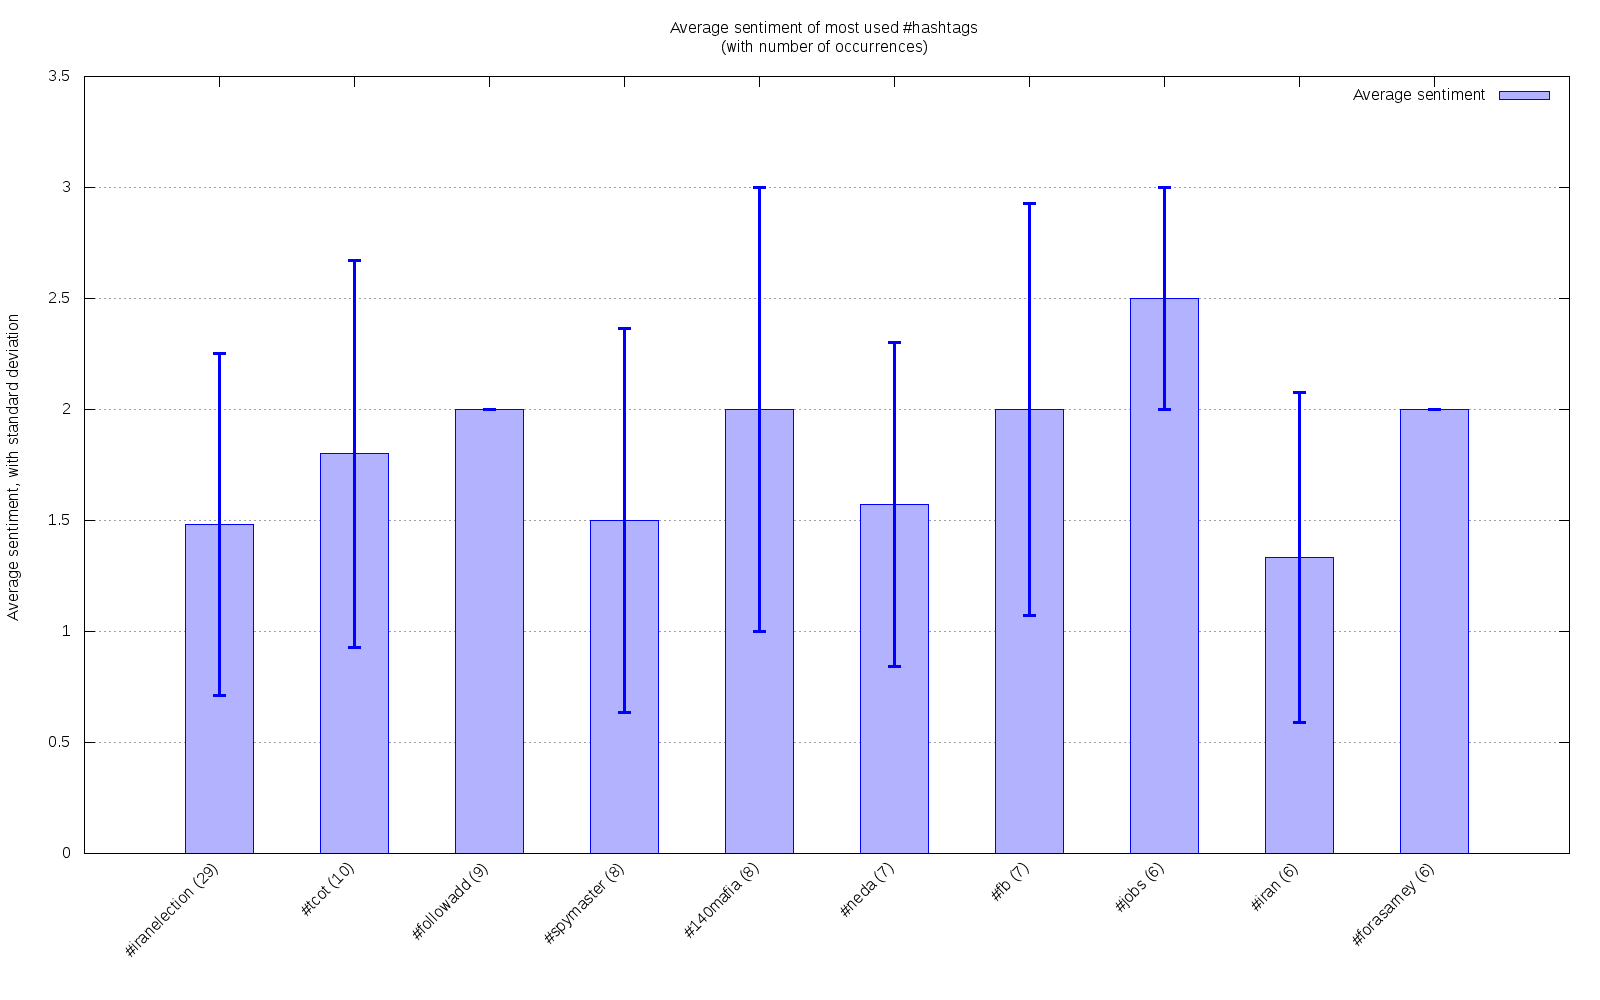
\includegraphics[width=\textwidth]{sentiment}
\end{center}
\captionof{figure}{The average sentiment value and standard deviation of the ten
most popular hashtags in the dataset.}

\begin{center}
    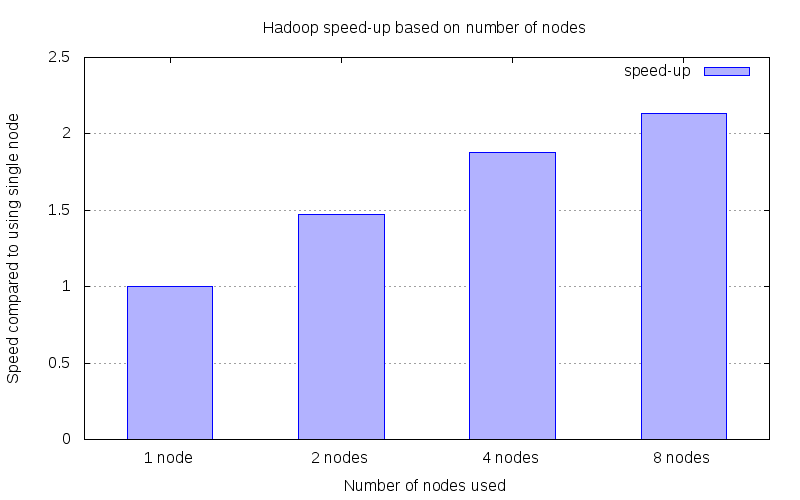
\includegraphics[width=\textwidth]{speedup}
\end{center}
\captionof{figure}{Speed up factor of the program when running on multiple nodes
compared to one node.}

\section{Conclusion}

As can be seen in the graphs presented above, the speed-up is not that
significant even when using eight nodes. This can be explained by the fact that
many other tasks were running at the same time on the system while our program
was running. Another explanation is the fact that our dataset is not large
enough to get the maximum speed-up from hadoop.


% =================================== REFERENCES ===================================

%\clearpage
%\bibliographystyle{unsrt}
%\bibliography{bib}

\end{document}
